\documentclass{standalone}
\usepackage{tikz}
\usepackage{amsmath}

\begin{document}

\tikzset{every picture/.style={line width=0.75pt}} %set default line width to 0.75pt

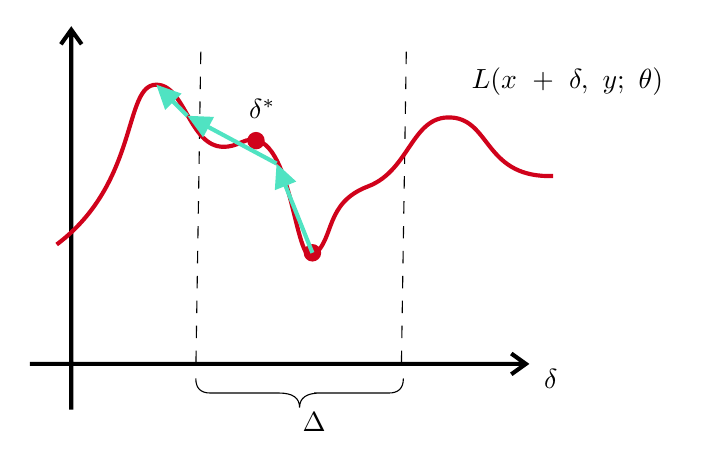
\begin{tikzpicture}[x=0.75pt,y=0.75pt,yscale=-1,xscale=1]
%uncomment if require: \path (0,209.36666870117188); %set diagram left start at 0, and has height of 209.36666870117188

%Shape: Axis 2D [id:dp8362083663235863]
\draw [color={rgb, 255:red, 0; green, 0; blue, 0 }  ,draw opacity=1 ][line width=1.5]  (177,165) -- (416,165)(197,4) -- (197,187) (409,160) -- (416,165) -- (409,170) (192,11) -- (197,4) -- (202,11)  ;
%Straight Lines [id:da16507939269124094]
\draw  [dash pattern={on 4.5pt off 4.5pt}]  (259.42,14.57) -- (257,169.18) ;


%Straight Lines [id:da38834176266730325]
\draw  [dash pattern={on 4.5pt off 4.5pt}]  (358.42,14.57) -- (356,169.18) ;


%Shape: Brace [id:dp915392662431817]
\draw   (257,172.02) .. controls (257,176.69) and (259.33,179.02) .. (264,179.02) -- (297,179.02) .. controls (303.67,179.02) and (307,181.35) .. (307,186.02) .. controls (307,181.35) and (310.33,179.02) .. (317,179.02)(314,179.02) -- (350,179.02) .. controls (354.67,179.02) and (357,176.69) .. (357,172.02) ;
%Shape: Circle [id:dp8402919319724125]
\draw  [draw opacity=0][fill={rgb, 255:red, 208; green, 2; blue, 27 }  ,fill opacity=1 ] (281.79,57.43) .. controls (281.79,55.11) and (283.68,53.23) .. (286,53.23) .. controls (288.32,53.23) and (290.21,55.11) .. (290.21,57.43) .. controls (290.21,59.76) and (288.32,61.64) .. (286,61.64) .. controls (283.68,61.64) and (281.79,59.76) .. (281.79,57.43) -- cycle ;
%Shape: Circle [id:dp15262915345215888]
\draw  [draw opacity=0][fill={rgb, 255:red, 208; green, 2; blue, 27 }  ,fill opacity=1 ] (308.98,111.47) .. controls (308.98,109.14) and (310.86,107.26) .. (313.18,107.26) .. controls (315.51,107.26) and (317.39,109.14) .. (317.39,111.47) .. controls (317.39,113.79) and (315.51,115.68) .. (313.18,115.68) .. controls (310.86,115.68) and (308.98,113.79) .. (308.98,111.47) -- cycle ;
%Curve Lines [id:da9436569690680264]
\draw [color={rgb, 255:red, 208; green, 2; blue, 27 }  ,draw opacity=1 ][line width=1.5]    (189.98,107.47) .. controls (229.98,77.47) and (221.98,30.47) .. (237.98,30.47) .. controls (253.98,30.47) and (254.02,69.98) .. (279,58.23) .. controls (303.98,46.47) and (303.98,120.47) .. (313.98,112.47) .. controls (323.98,104.47) and (318.98,87.47) .. (339.98,79.47) .. controls (360.98,71.47) and (360.98,43.37) .. (381.98,46.47) .. controls (399.18,49.47) and (397.18,75.47) .. (429.18,74.47) ;


%Straight Lines [id:da011379826508587376]
\draw [color={rgb, 255:red, 80; green, 227; blue, 194 }  ,draw opacity=1 ][line width=1.5]    (313.18,111.47) -- (297.03,71.23) ;
\draw [shift={(295.92,68.45)}, rotate = 428.13] [fill={rgb, 255:red, 80; green, 227; blue, 194 }  ,fill opacity=1 ][line width=1.5]  [draw opacity=0] (11.61,-5.58) -- (0,0) -- (11.61,5.58) -- cycle    ;

%Straight Lines [id:da053371808091445816]
\draw [color={rgb, 255:red, 80; green, 227; blue, 194 }  ,draw opacity=1 ][line width=1.5]    (295.92,68.45) -- (255.56,46.86) ;
\draw [shift={(252.92,45.45)}, rotate = 388.14] [fill={rgb, 255:red, 80; green, 227; blue, 194 }  ,fill opacity=1 ][line width=1.5]  [draw opacity=0] (11.61,-5.58) -- (0,0) -- (11.61,5.58) -- cycle    ;

%Straight Lines [id:da16718105434047426]
\draw [color={rgb, 255:red, 80; green, 227; blue, 194 }  ,draw opacity=1 ][line width=1.5]    (252.92,45.45) -- (240.09,32.59) ;
\draw [shift={(237.98,30.47)}, rotate = 405.08000000000004] [fill={rgb, 255:red, 80; green, 227; blue, 194 }  ,fill opacity=1 ][line width=1.5]  [draw opacity=0] (11.61,-5.58) -- (0,0) -- (11.61,5.58) -- cycle    ;


% Text Node
\draw (436,29.02) node   {$L( x\ +\ \delta ,\ y;\ \theta )$};
% Text Node
\draw (428,172.02) node   {$\delta $};
% Text Node
\draw (314,193.02) node   {$\Delta $};
% Text Node
\draw (289,42.02) node   {$\delta ^{*}$};

\end{tikzpicture}

\end{document}
